\chapter{Detailed Design}
\label{chap:detailed-design}

% This section will form the bulk of the report. Here you should include
% design decisions and tradeoffs as well as any detailed technical drawings
% such as circuit diagrams, flow charts, etc.  If these are particularly large
% they may be placed in an appendix, but should be referenced in this section.

% It is here that you really get into the details of why your project is
% designed the way it is.  Tradeoffs are made in a number of areas and a good
% way to organize this section is to figure out what the most important
% tradeoffs are and explain each of them with a few paragraphs.

% This is a section that will evolve as the project nears completion, but its
% writing could be started at the beginning of the semester.  I'll be happy to
% give feedback on whatever you are able to produce for this section during the
% semester, while recognizing that some elements will be subject to change or
% impossible to write up until the final project is completed.

\section{Power Supply Unit}
Due to the volatile nature of automotive electrical systems, an exceptionally stable and 
resilient power supply is required for this project.  As mentioned previously, large
transient voltages are not uncommon in automotive environments, so the electronics must
be designed to survive such conditions.  For these reasons, the power supply employs 
a number of protection techniques and switching regulators to provide safe, consistent 
power to the remaining circuitry.

The input stage of the power supply provides over-, under-, and reverse-voltage
protection.  A control chip from Linear Technology \cite{ltc4365ds} is used to drive two pass
field-effect transistors (FETs) if the supply voltage is between 3.5 and 18 volts.  If the supply voltage
is outside this range, the FETs are turned off and the circuitry is
protected.  Large transient-voltage-suppression (TVS) diodes are also present to
protect against severe ($\pm 100$V) transients.  The output of this stage includes
large bulk capacitors to handle brown-outs.

The second portion of the power supply includes a dual buck switching regulator
to provide 3.3V and 5V at 3A apiece.  This portion of the supply must support 
the highest loads during normal operation.  The Raspberry Pi, AVR 
microcontroller, and vacuum-fluorescent display are all powered from 5V and 
require up to 2A.  The USB-to-UART \cite{ft2232hds} and OBD-to-UART \cite{stn1110ds} converters both use 3.3V at 
close to 500mA.  A buck topology was chosen since the supply voltage will be
above 5V except during severe brown-out conditions.

The third and final portion of the power supply uses a buck-boost switching
regulator \cite{ltc3115ds} to supply 12V at 1.5A.  This voltage is used to support several
OBD protocols.  While the raw voltage from the car itself could be used
for this purpose, more protection would be required.  This supply also allows
for different displays that may require 12V.  A buck-boost topology was chosen
because the input voltage can drop well below 12V, though most of the time it is
around 14V.

The power supply was designed as a 4-layer PCB, of which most layers are grounded 
in order to provide heat-sinking and shielding from high-frequency switching signals.

\begin{figure}[h]
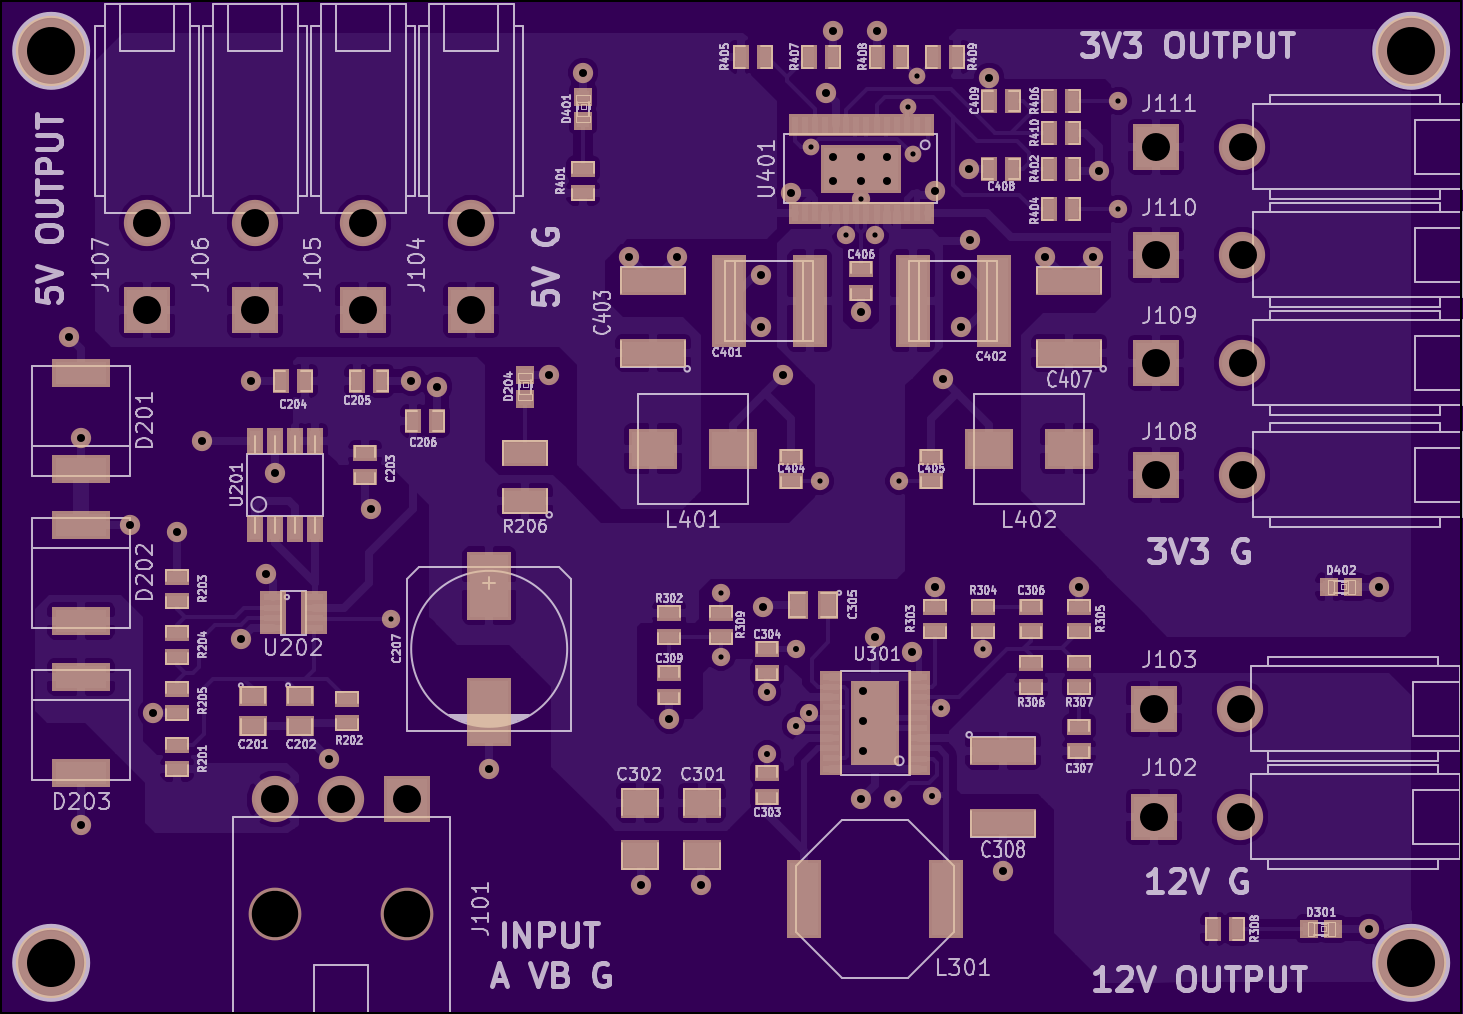
\includegraphics[width=\textwidth]{img/psu_render_top.png}
\caption{Top of the PSU board}
\label{fig:psu render}
\end{figure}

\section{Main Board}
The main board handles all functions not performed by the Raspberry Pi.  It will
provide an interface to the vehicle, receive data from the Raspberry Pi and 
display that data to the VFD.  External inputs are also provided for future 
development.  The main board was designed as a 4-layer PCB.

\subsection{Microcontroller}
An Atmel AVR ATmega32U4 \cite{atmega32u4ds} was chosen as the microcontroller to drive the VFD.  This
controller provides sufficient memory and processing power to handle this task. 
It is also used to handle switch inputs for changing brightness, display modes,
and other options.  The AVR can also output to a character LCD
for debugging.  It will communicate with the Raspberry Pi via UART.

\subsection{STN1110}
An STN1110 was selected as the interface chip between the Raspberry Pi and the 
vehicle.  The STN and its supporting circuitry handle all of the standard OBD
protcols and communicate via UART.  This chip is considered an improvement over
the ubiquitous ELM327 used in many USB and Bluetooth adapters.  The STN provides
more functionality than the ELM and includes an additional instruction set that
can streamline higher-level software. A datasheet for this device is available
at \cite{stn1110ds}.

\subsection{FTDI USB to UART}
To easily connect both the AVR and STN to the Raspberry Pi, an FTDI FT2232H UART 
to USB converter was included on the main board.  This chip will enumerate on the
Raspberry Pi as two virtual serial ports.  These ports are very easy to interface
with via C and provide an easy communication method.  The chip supports UART baud
rates up to 1MBaud, which is sufficiently fast for all operations in this project.
A datasheet for this device is available at \cite{ft2232hds}.

\begin{figure}[h]
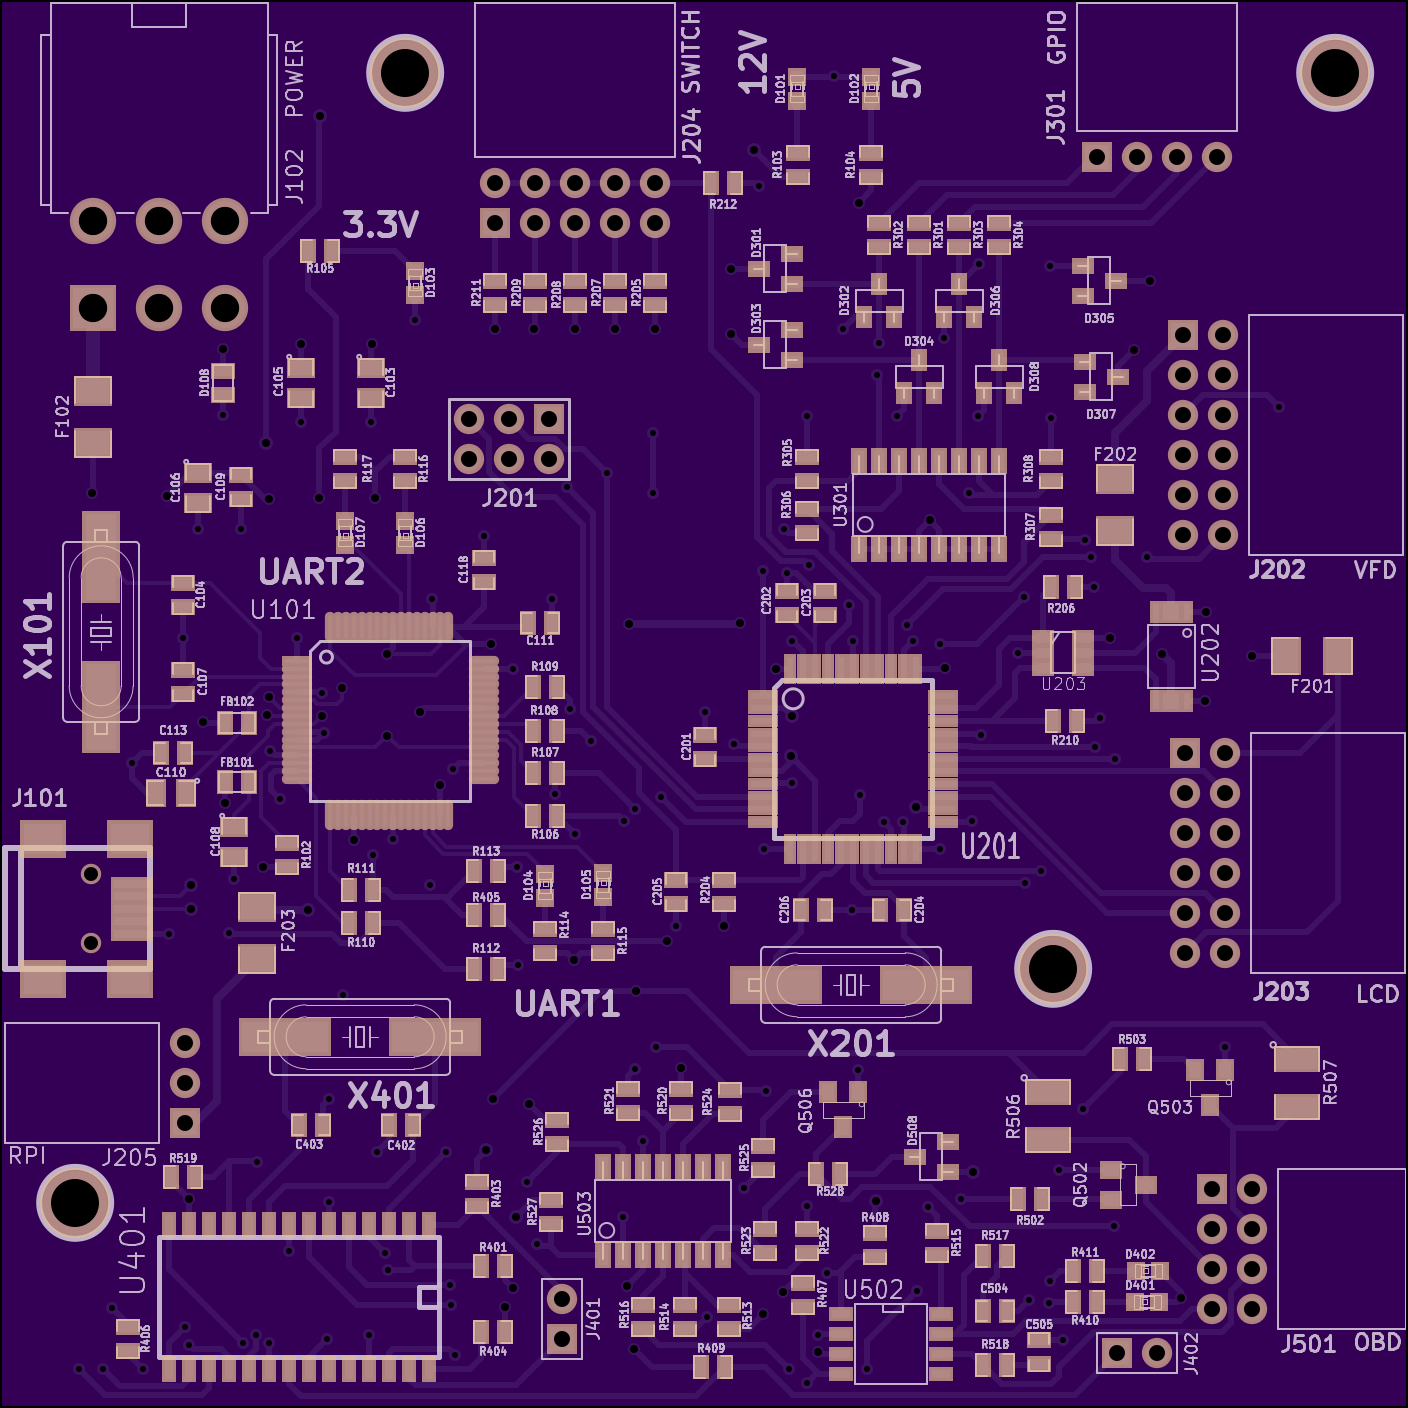
\includegraphics[width=\textwidth]{img/main_render_top.png}
\caption{Top of the main board}
\label{fig:main render}
\end{figure}

\section{Raspberry Pi}
\label{sec:raspi-design}

A Raspberry Pi computer was chosen to be high-level platform for this system
because of its popularity and ease of use. The Raspberry Pi is connected to the
main board via USB, and delegates the tasks of gathering and displaying data
to the main board.

\subsection{Operating System}
We chose Rasbian to be the operating system for the Raspberry Pi because it is the
most used and well-known operating system for the Raspberry Pi. We wanted to focus
on designing the overall
system, not on wrestling with an obscure operating system. We prioritized ease
of development.

\section{Software}
The software for the system was prototyped in Python 2.7.5, and then finally
implemented in C$++$. Python was chosen
because it is the language of choice for the Raspberry Pi, and allows us to
quickly and easily develop the high-level system software. Version 2.7.5 was
chosen for compatibility with the PySerial library, which the software uses to
communicate over USB.

The code that runs on the Raspberry Pi is very simple. It pulls speed and RPM
from the OBD subsystem on the main board, and pushes that data to the AVR
subsystem. The microcontroller in the AVR subsystem then displays that data
on the display.

The Raspberry Pi is almost useless in the final implementation of the system, and
could be removed for a main board that could control both subsystems from its
microcontoller. The Pi could also be used as a platform for other improvements.

Source code for the system (as well as source code for this report) can be
found at \url{https://github.com/Cantido/vehiclehud}.

\section{Optics}
\subsection{Main Display}
For the main display, a vacuum fluorescent display (VFD) was chosen.  VFDs offer
extreme brightness, suitable for a system that will be used in daylight.  The
one chosen for this project was made by Noritake and offers 128x64 pixels.  
While this resolution is not fantastic, it does provide the ability to make a
nice, clean display.  The AVR microcontroller on the main board communicates 
with the VFD via a proprietary serial interface.  Noritake provides a C$++$ 
library for use with AVRs.

\subsection{Focusing Mirror}
In order for this project to be a true ``heads-up'' 
display, the image must be focused at infinity.  To accomplish this, a 
parabolic reflector was used.  Parabolic reflectors are often used in solar
collectors; light from the sun is reflected off the parabolic surface and
focused at the focal point of the parabola.  This process works in reverse 
as well: if the display is placed at the focal point of the parabola, the
light from the display will be collimated (all rays made parallel) thus
focusing the image at infinity.  Once reflected onto the windshield, the
display's image will appear to be at inifnity.

To create a parabolic mirror, a base was made from laser-cut acrylic slices.
These slices were bolted together and covered with a mirror-coated film.  While
this did create a mirror that would focus the image at inifity, it was rather
rough around the edges, both literally and figuratively.  The edges of the mirror
were not perfect and created some distorion.  A model of the mirror assembly is 
shown in figure~\ref{fig:mirror-render}.

\begin{figure}[h]
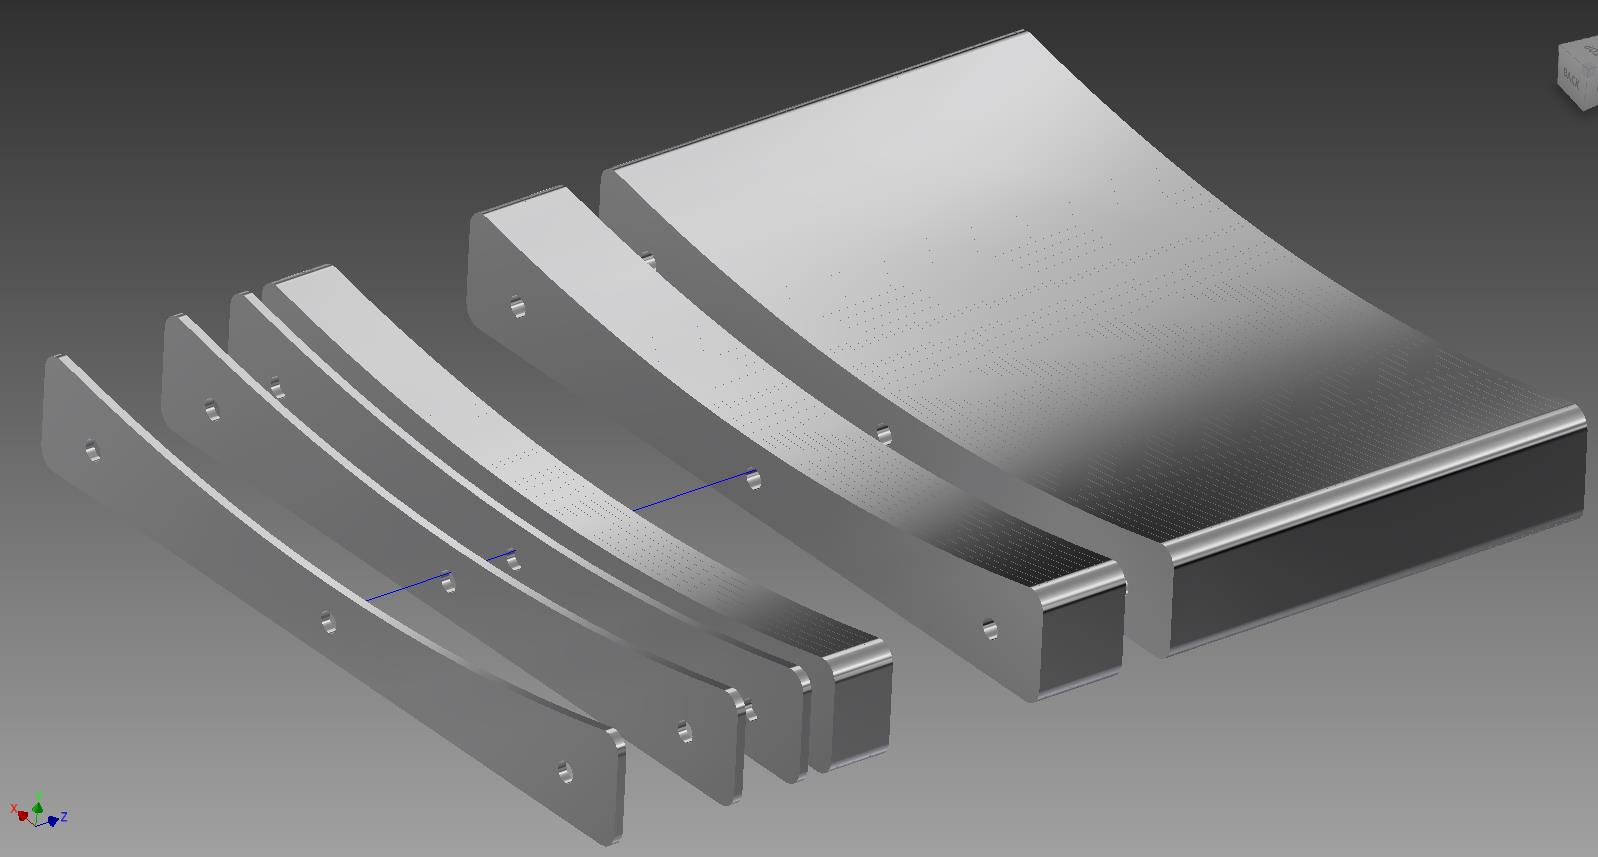
\includegraphics[width=\textwidth]{img/mirror_render.jpg}
\caption{Construction of the focusing mirror}
\label{fig:mirror-render}
\end{figure}
